
%(BEGIN_QUESTION)
% Copyright 2015, Tony R. Kuphaldt, released under the Creative Commons Attribution License (v 1.0)
% This means you may do almost anything with this work of mine, so long as you give me proper credit

\noindent

\vskip 5pt



\vskip 5pt
\begin{center}
\textbf{Arbeidsoppdrag reguleringsteknikk}
\vskip 5pt 
\vskip 5pt 
\end{center}

\vskip 10pt 
\textbf{Introduksjon}

\vskip 5pt 
I dette arbeidsoppdraget skal du gjøre følgende:
\begin{itemize}[noitemsep]
	\item Koble opp stasjonen i henhold til P \&ID
	\item Programmere stasjonen slik at den virker i henhold til spesifikasjon
	\item Lage HMI i henhold til spesifikasjon. 
	\item Optimalisere funksjon og instrumenter. 
\end{itemize}

\textbf{Generelt om stasjon 05}

Stasjon 05 er en reguleringsmodell, tiltenkt for undervisning i reguleringsteknikk.  

Stasjonen inneholder to vanntanker koblet sammen med rør, reguleringsventil og pumpe. Det pumpes opp vanntrykk med en pumpe og strømningen inn i tanken reguleres med en ventil. Det er mulig å koble inn en membrantank mellom pumpe og ventil for å kunne oppta trykkenergi.  

Strømning inn i tanken måles med et paddel wheel strømningsmåler.   

Instrumenteringen på stasjonen består nå av:  

Paddel Wheel Strømningsmåler 

Frekvensomformerstyrt pumpe 

Reguleringsventil. 

Wago PFC 200 PLS (med Codesys runtime) 


Enkle funksjoner på stasjonen skal kunne styres fra styrepanel på stasjonen. I vanlig bruk skal det være mulig for elever å koble seg opp til stasjonen v.h.a. nettleser og styre den med HMI

%$$\includegraphics[width=13cm]{i04824x01.eps}$$\\


\textbf{Generelt om oppgaven }

Før selve oppgaven påbegynnes skal du utføre en sjekk av utstyret for så å rive ned alle ledninger og kabler. 

I hovedoppgaven skal du bygge opp, programmere stasjonen, laget et bruker grensesnitt, optimalisere og lage dokumentasjon på stasjonen. 

 

 Hovedmomenter i oppgaven vil være: 
\begin{itemize}[noitemsep]
	\item Bygge maskinstyring i kapsling.  
	\item Legge kabel til alt utstyr og implementere dette i styresystemet
	\item Legge opp tilførselskabel til stasjonen, men tilhørende montering av kabelstige 
	\item Programmere styresystem for modellen 
	\item Lage HMI for stasjonen tilpasset opplæring i reguleringsteknikk og koble stasjonen til  nettverk for tilgang til HMI.  
	\item Kalibrering av instrumenter og optimalisering. 
	\item Utarbeiding av dokumentasjon for stasjonen. 
\end{itemize}



 

 Design krav:  
\begin{itemize}[noitemsep]
	\item Frekvensomformer skal tilkobles styresystemet v.h.a. feltbuss. Sikkerhetsrelaterte deler av styresystemet tilkobles frekvensomformeren sin STO funksjon.  
	\item Det skal brukes sikkerhetsrele til sikkerhetsrelaterte deler av styresystemet
	\item Nivåbryter for høyt nivå i tanken skal tilkobles sikkerhetsrelaterte deler av styresystemet som stopper pumpen.
	\item Det skal være avstenging for all energiforsyning på stasjonen.  
	\item HMI skal i størst mulig grad designes etter prinsippene i «The-High-Performance-HMI-Overview-Part-1-PAS-Inc».  
	\item Enkle funksjoner på stasjonen skal kunne styres fra styrepanel på stasjonen. I vanlig bruk skal det være mulig for elever å koble seg opp til stasjonen v.h.a. nettleser og styre den med HMI.  
\end{itemize}


\textbf{Stasjonens fuksjonalitet}

Du skal koble sammen og programmere stajonen slik at den virker på følgende måte:

\vskip 5pt 

Når anlegget spenningsettes må en trykke en resett knapp som aktiverer et grønt «klar» lys. Dette symboliserer at stasjonen er klar til å tas i bruk. Når Sikkerhetsrelaterte deler av styresystemet utløses slukker klar lyset. Når årsaken er utbedret må en igjen trykke resett for å gjøre systemet klart for start.  

\vskip 5pt 
Alarm funksjonalitet: 

Det skal gis alarm ved følgende tilfeller: 

Ved nivå over 90 % aktiveres en H alarm 

Ved strømning over 90% aktiveres en H alarm 

Ved trykk over 80 % aktiveres en H alarm 

\vskip 5pt 
Alarmer skal ha bekreft og reset funksjonalitet. Ved alarm blinker alarm lyset. Når bekreft trykkes lyser det konstant. Når alarm tilstand opphører kan en resette alarmen.  

\vskip 5pt 
Styring av stasjonen gjøres fra HMI i et web grensesnitt.

\vskip 5pt 
Stasjonen skal ha tre funksjonsmodus: 
\begin{itemize}[noitemsep]
	\item Tilbakekoblet regulering med frekvensomformerstyrt pumpe
	\item Kaskadekoblet regulering med ventil (pumpe brukes til å generere forstyrrelser)
	\item Tilbakekoblet regulering av nivå med ventil med konstant pumpetrykk). 
\end{itemize}

\vskip 5pt 


Modus velges med en vri bryter på fronten. Når ny modus velges skal HMI skjerm automatisk bytte til skjermbilde som er tilpasset den aktuelle modus.   

\vskip 5pt 
\textbf{I tilbakekoblet regulering:} 
\begin{itemize}[noitemsep]
	\item Det byttes automatisk til HMI bilde for tilbakekoblet regulering 
	\item Nivå i stasjonen reguleres med ventil.  
	\item Reguleringen startes og stoppes ved hjelp av trykknapper.   
	\item HMI skal vise en forenklet P \& ID av anlegget og gjøre det mulig å optimalisere reguleringen ved hjelp av sprangresponstest på et trace.  
	\item Det skal være et valg for om en ønsker å bruke DP-celle eller ultralydmåler som nivåmåler for reguleringen. Alle nødvendige innstillinger for en reguleringssløyfe skal kunne gjøres fra HMI-en 
	\item Settpunkt skal kunne justeres i hopp på 5\% med + / - knapper på skap.  

\end{itemize}


\textbf{I kaskademodus:}

\begin{itemize}[noitemsep]
	\item Det byttes automatisk til HMI bilde for kaskadekoblet regulering 
	\item Master sløyfen regulerer nivå i tanken. Slavesløyfen regulerer strømning inn i tanken. 
	\item Strømning reguleres med ventilen. 
	\item Pumpen genererer automatiske forstyrrelser for reguleringen. 
	\item Reguleringen startes og stoppes ved hjelp av trykknapper.   
	\item HMI skal vise en forenklet P \& ID av anlegget og gjøre det mulig å optimalisere reguleringen (Master og slave sløyfe) ved hjelp av sprangresponstest på et trace.  
	\item Det skal være et valg for om en ønsker å bruke DP-celle eller ultralydmåler som nivåmåler for reguleringen. Alle nødvendige innstillinger for en reguleringssløyfe skal kunne gjøres fra HMI-en 
	\item Settpunkt skal kunne justeres i hopp på 5\% med + / - knapper på skap.  

\end{itemize}


\textbf{I Konstant trykk modus:}

\begin{itemize}[noitemsep]
	\item Det byttes automatisk til HMI bilde for konstakt trykk modus 
	\item Pumpen regulerer konstant trykk før ventil som  i gjen regulerer nivå i tankten. 
	\item Reguleringen startes og stoppes ved hjelp av trykknapper.   
	\item HMI skal vise en forenklet P \& ID av anlegget og gjøre det mulig å optimalisere reguleringene ved hjelp av sprangresponstest på et trace.  
	\item Det skal være et valg for om en ønsker å bruke DP-celle eller ultralydmåler som nivåmåler for reguleringen. Alle nødvendige innstillinger for en reguleringssløyfe skal kunne gjøres fra HMI-en 
	\item Settpunkt skal kunne justeres i hopp på 5\% med + / - knapper på skap.  

\end{itemize}

\href{https://rfka-my.sharepoint.com/:u:/g/personal/fred-olav_mosdal_skole_rogfk_no/EewzybzUnq5PscHy_uJUvUMB3ufsOB417mgUkhGlC8yQrg?e=rPkbpf}{Eksempel program med PID i codesys}

\vskip 5pt 

\vskip 5pt 

$$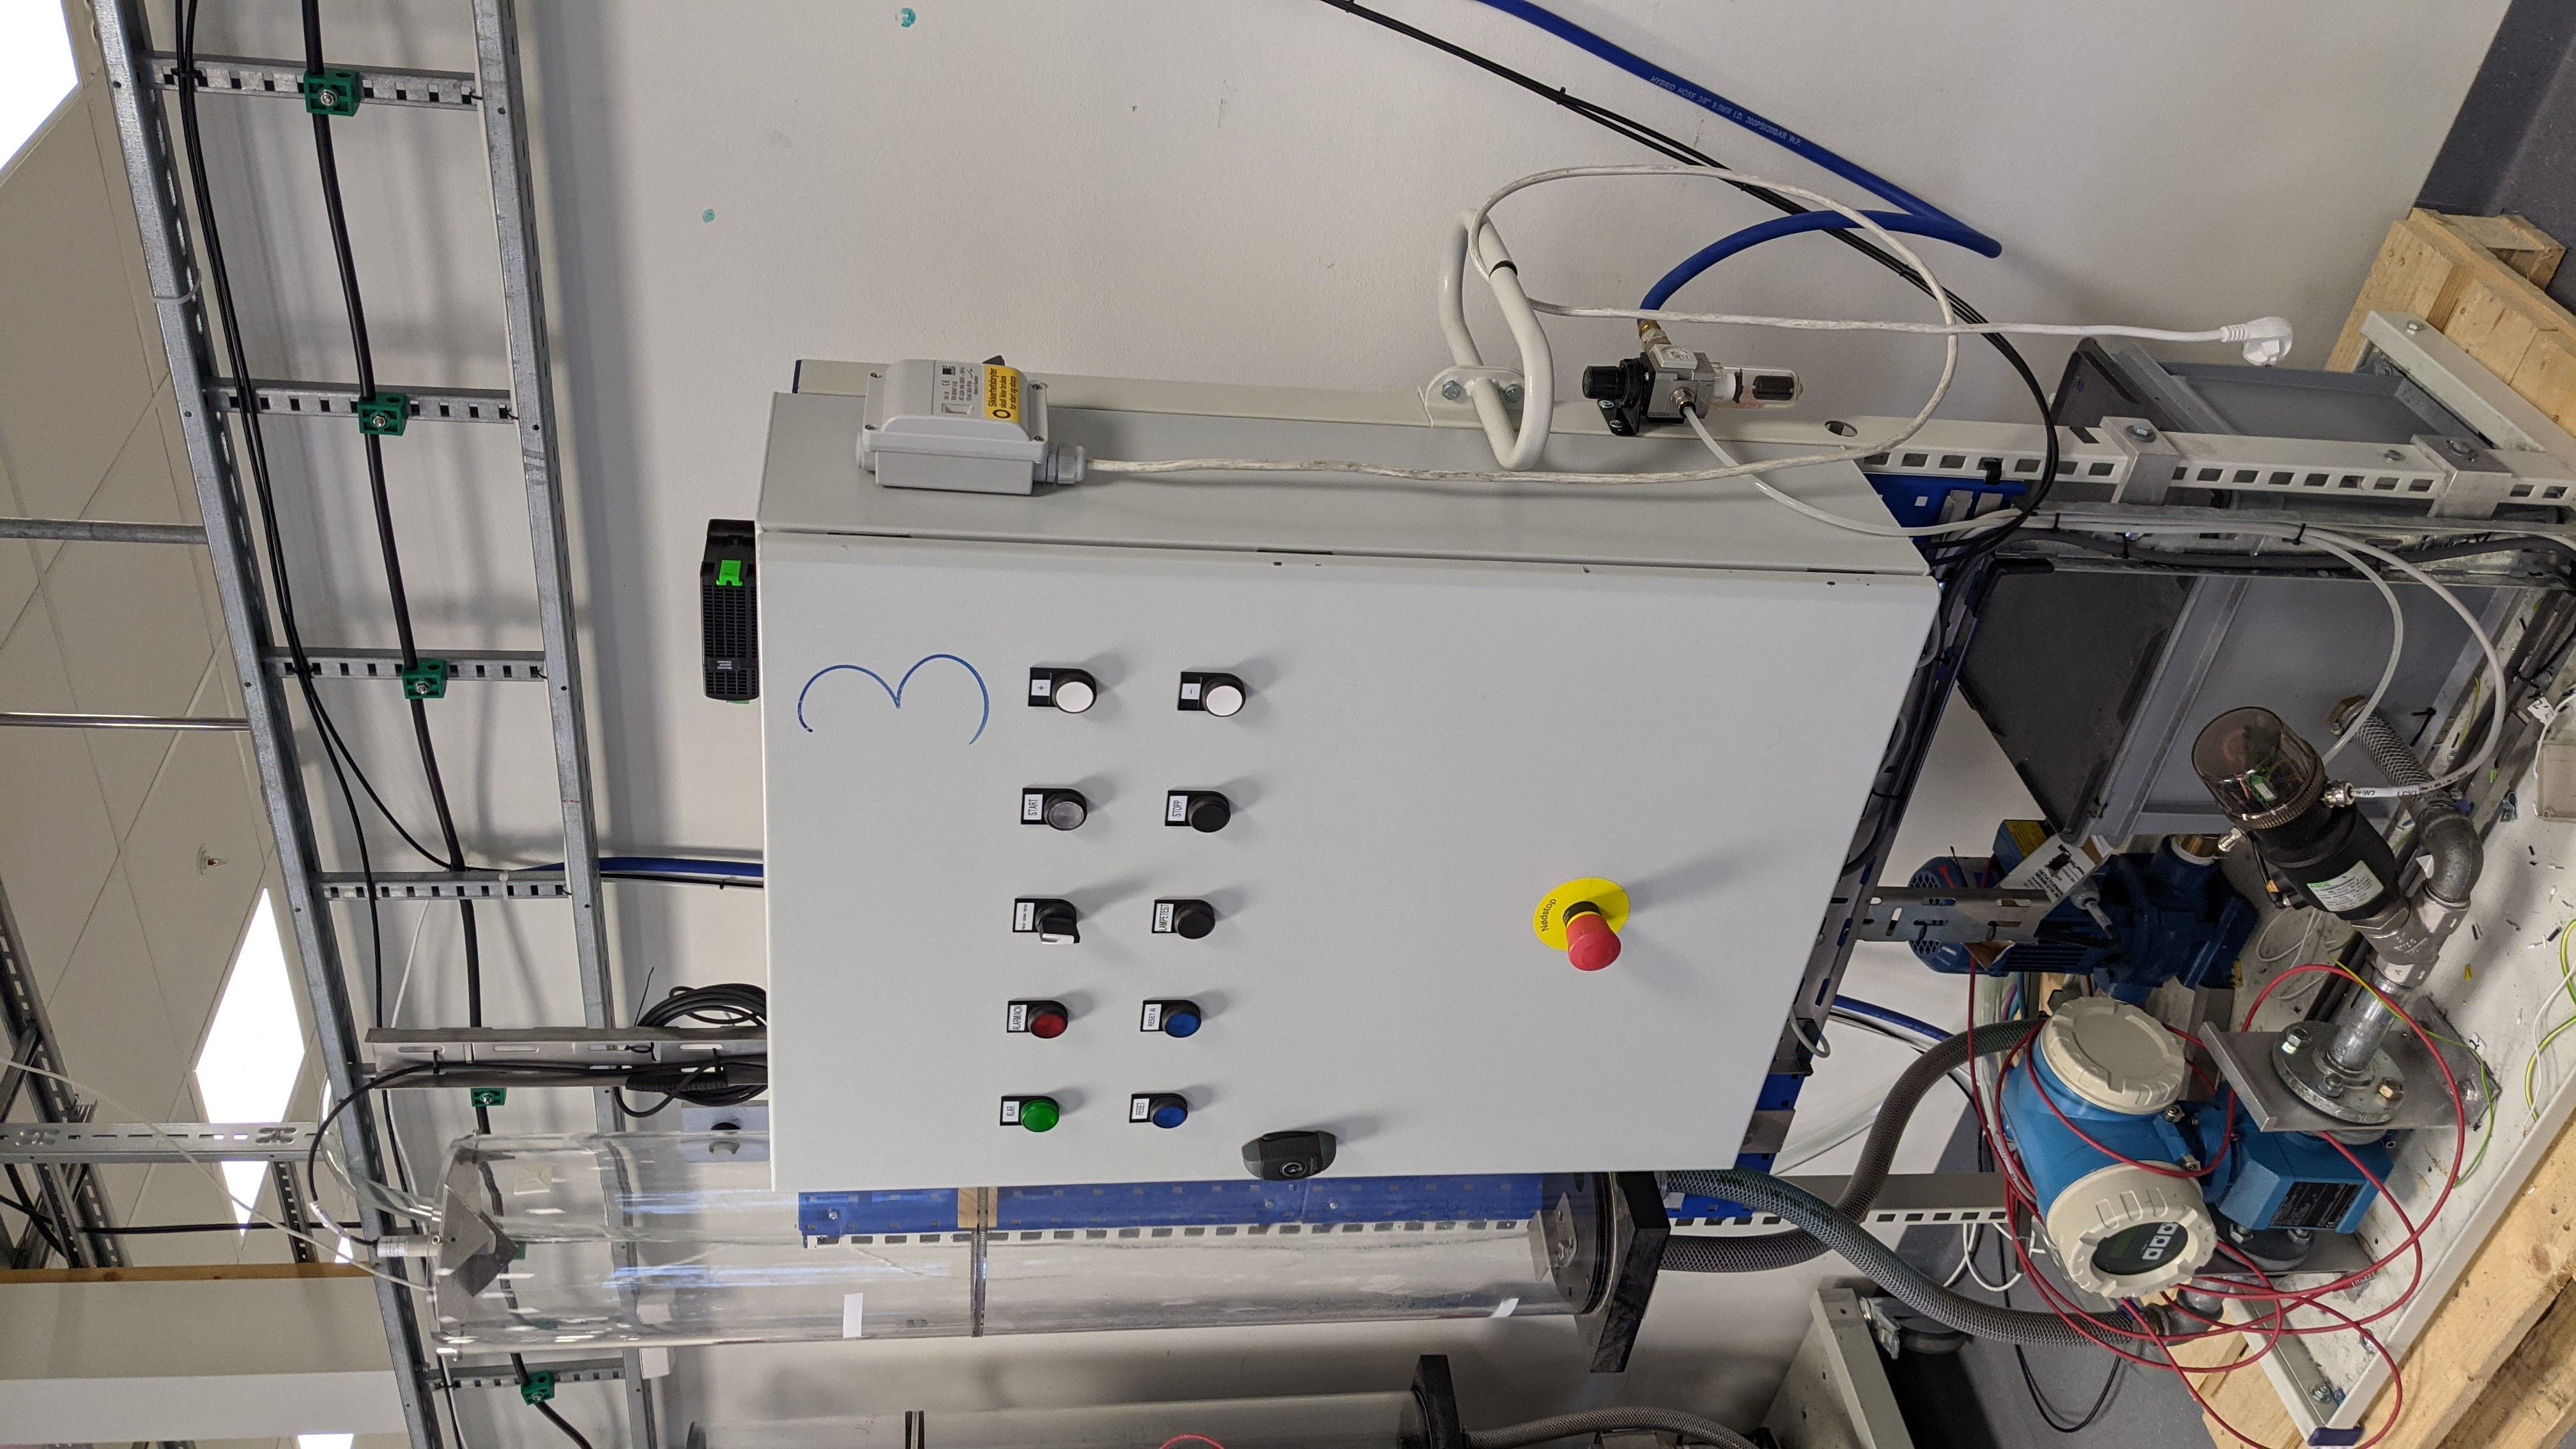
\includegraphics[width=10.5cm,angle=-90]{stasjon03x01.jpg},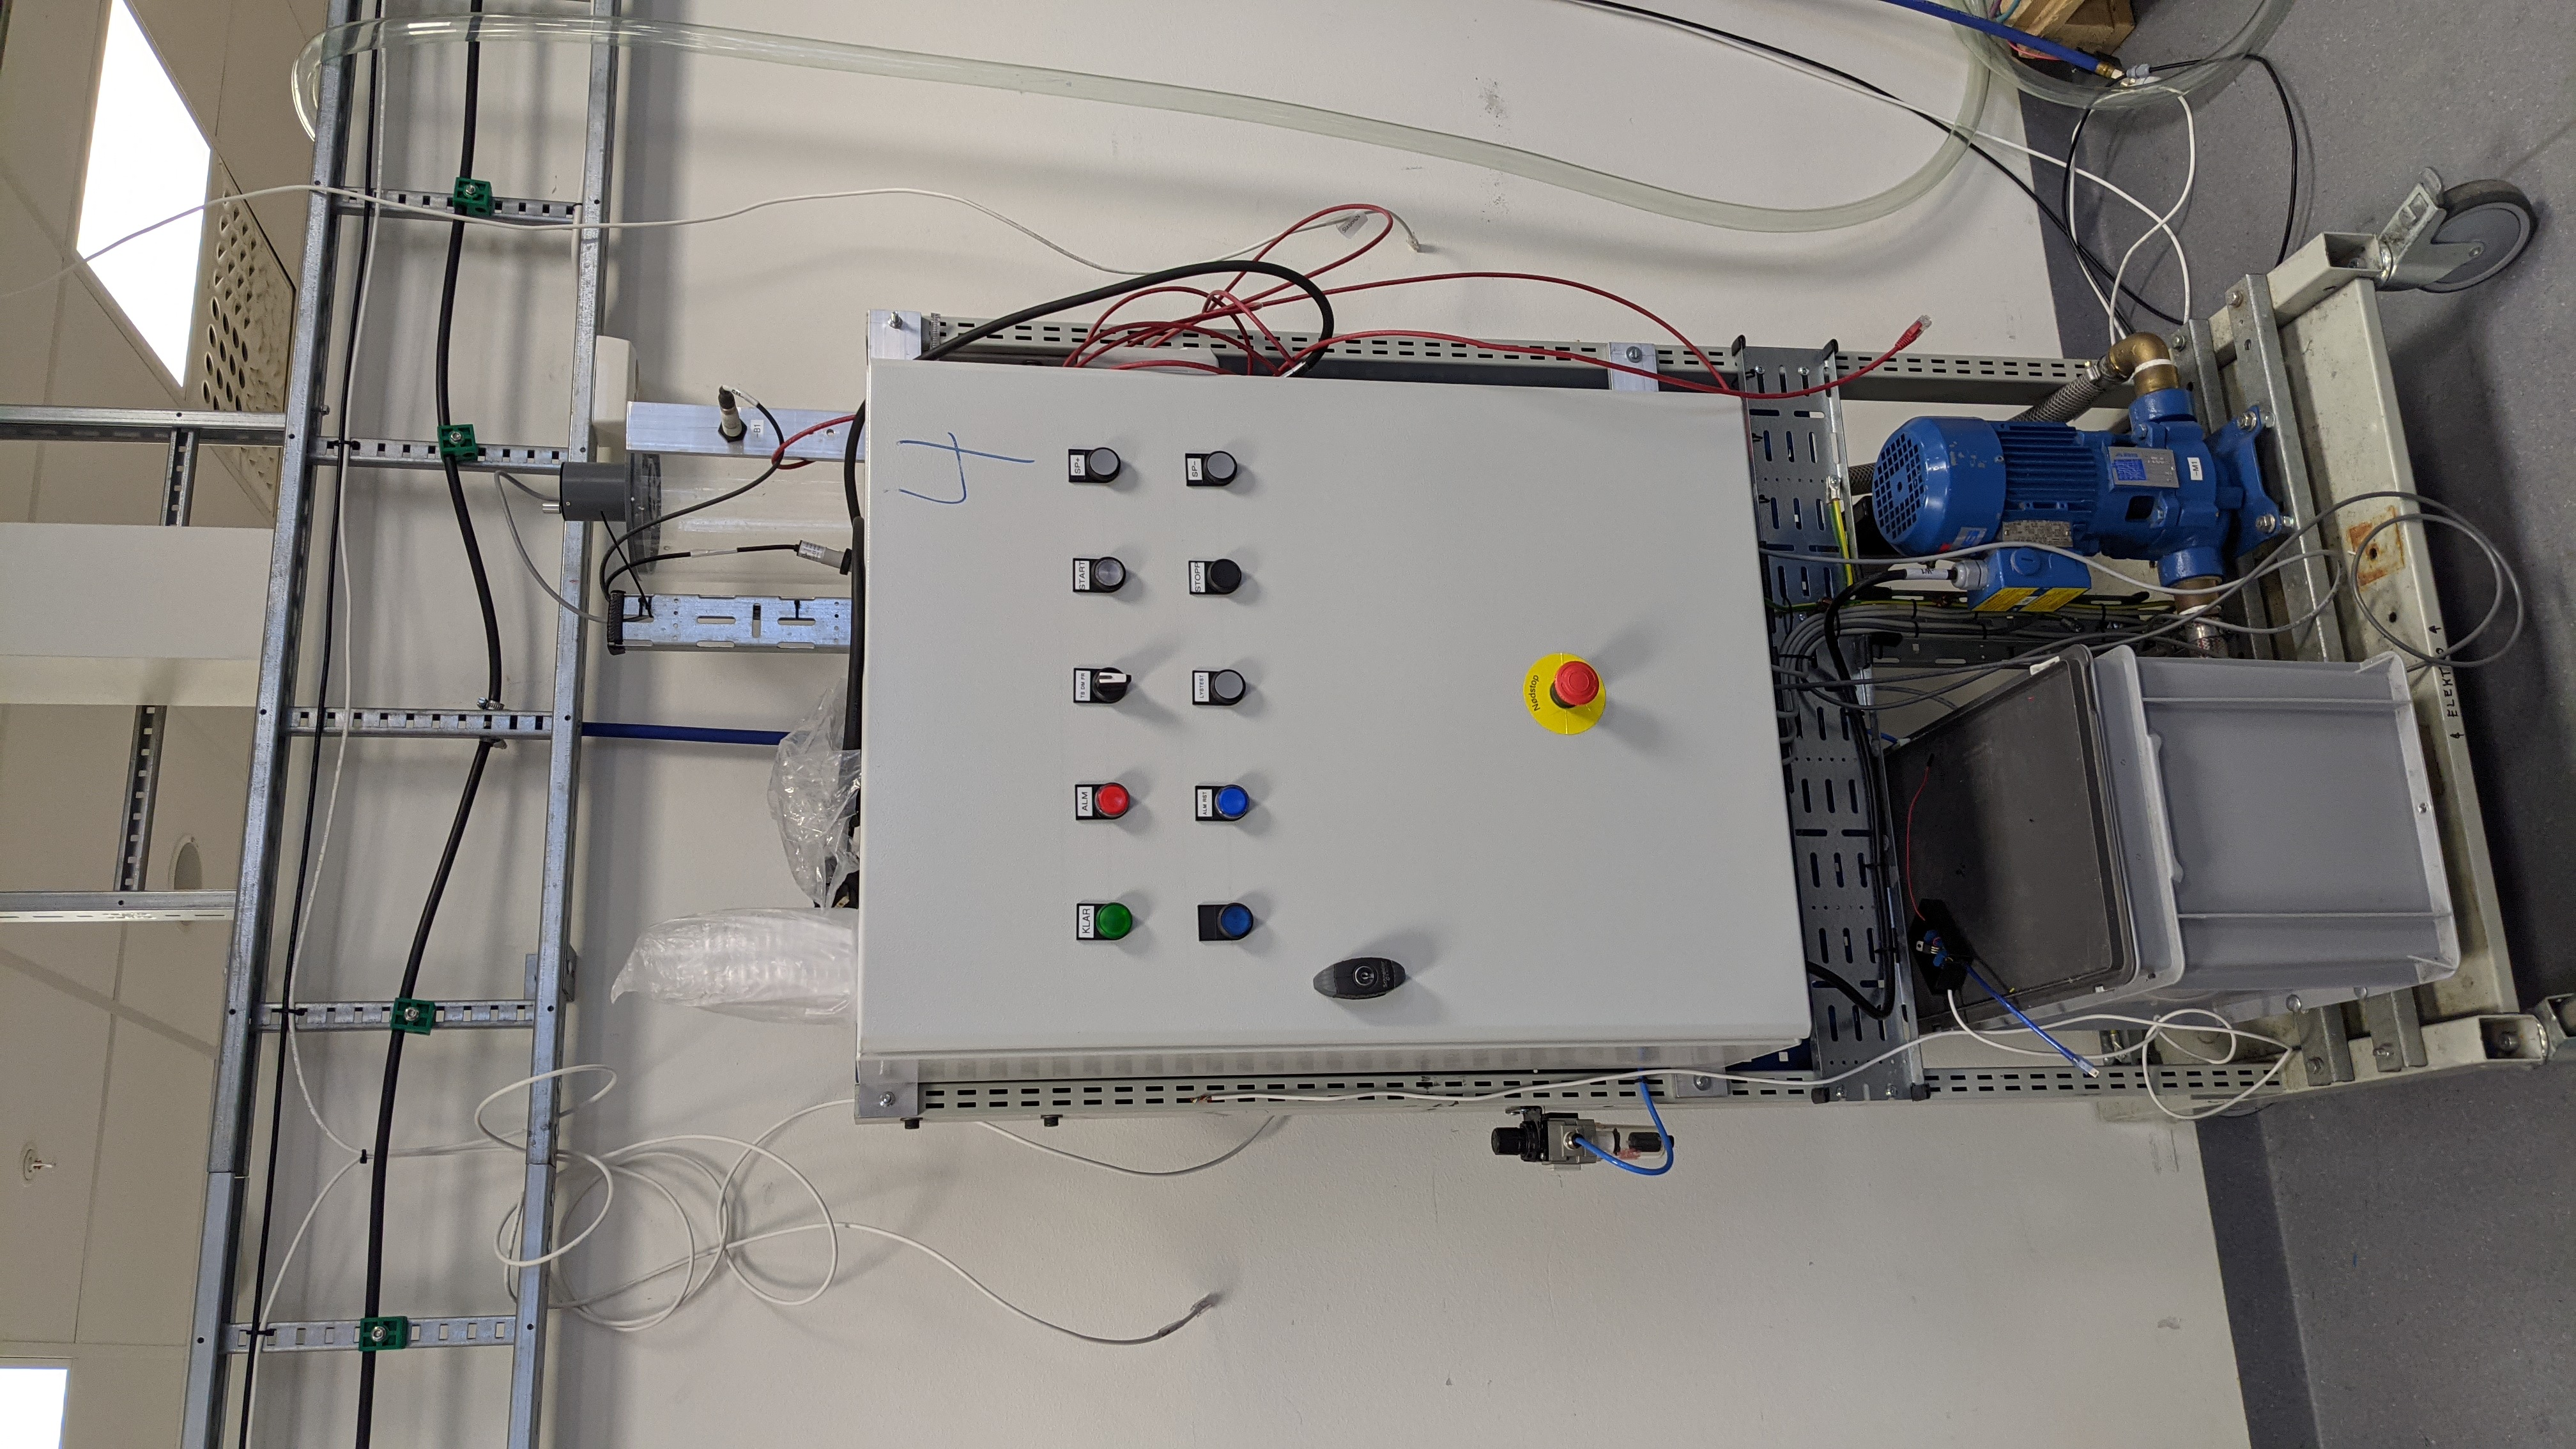
\includegraphics[width=10.5cm,angle=-90]{stasjon04x01.jpg}$$

\vskip 10pt 
\textbf{Teorioppgaver}
Leseoppgave:

\vskip 5pt 
\url {https://autofaget.no/closedloop/node2.html}
\vskip 5pt 
Oppgavehefte:
\vskip 5pt 
https://autofaget.no/pdfs/Regulering.pdf
\vskip 5pt 

\vskip 10pt 
\textbf{Planlegging}


\vskip 10pt 
\textbf{Gjennomføring}

\vskip 10pt 
\textbf{Dokumentasjon}

%$$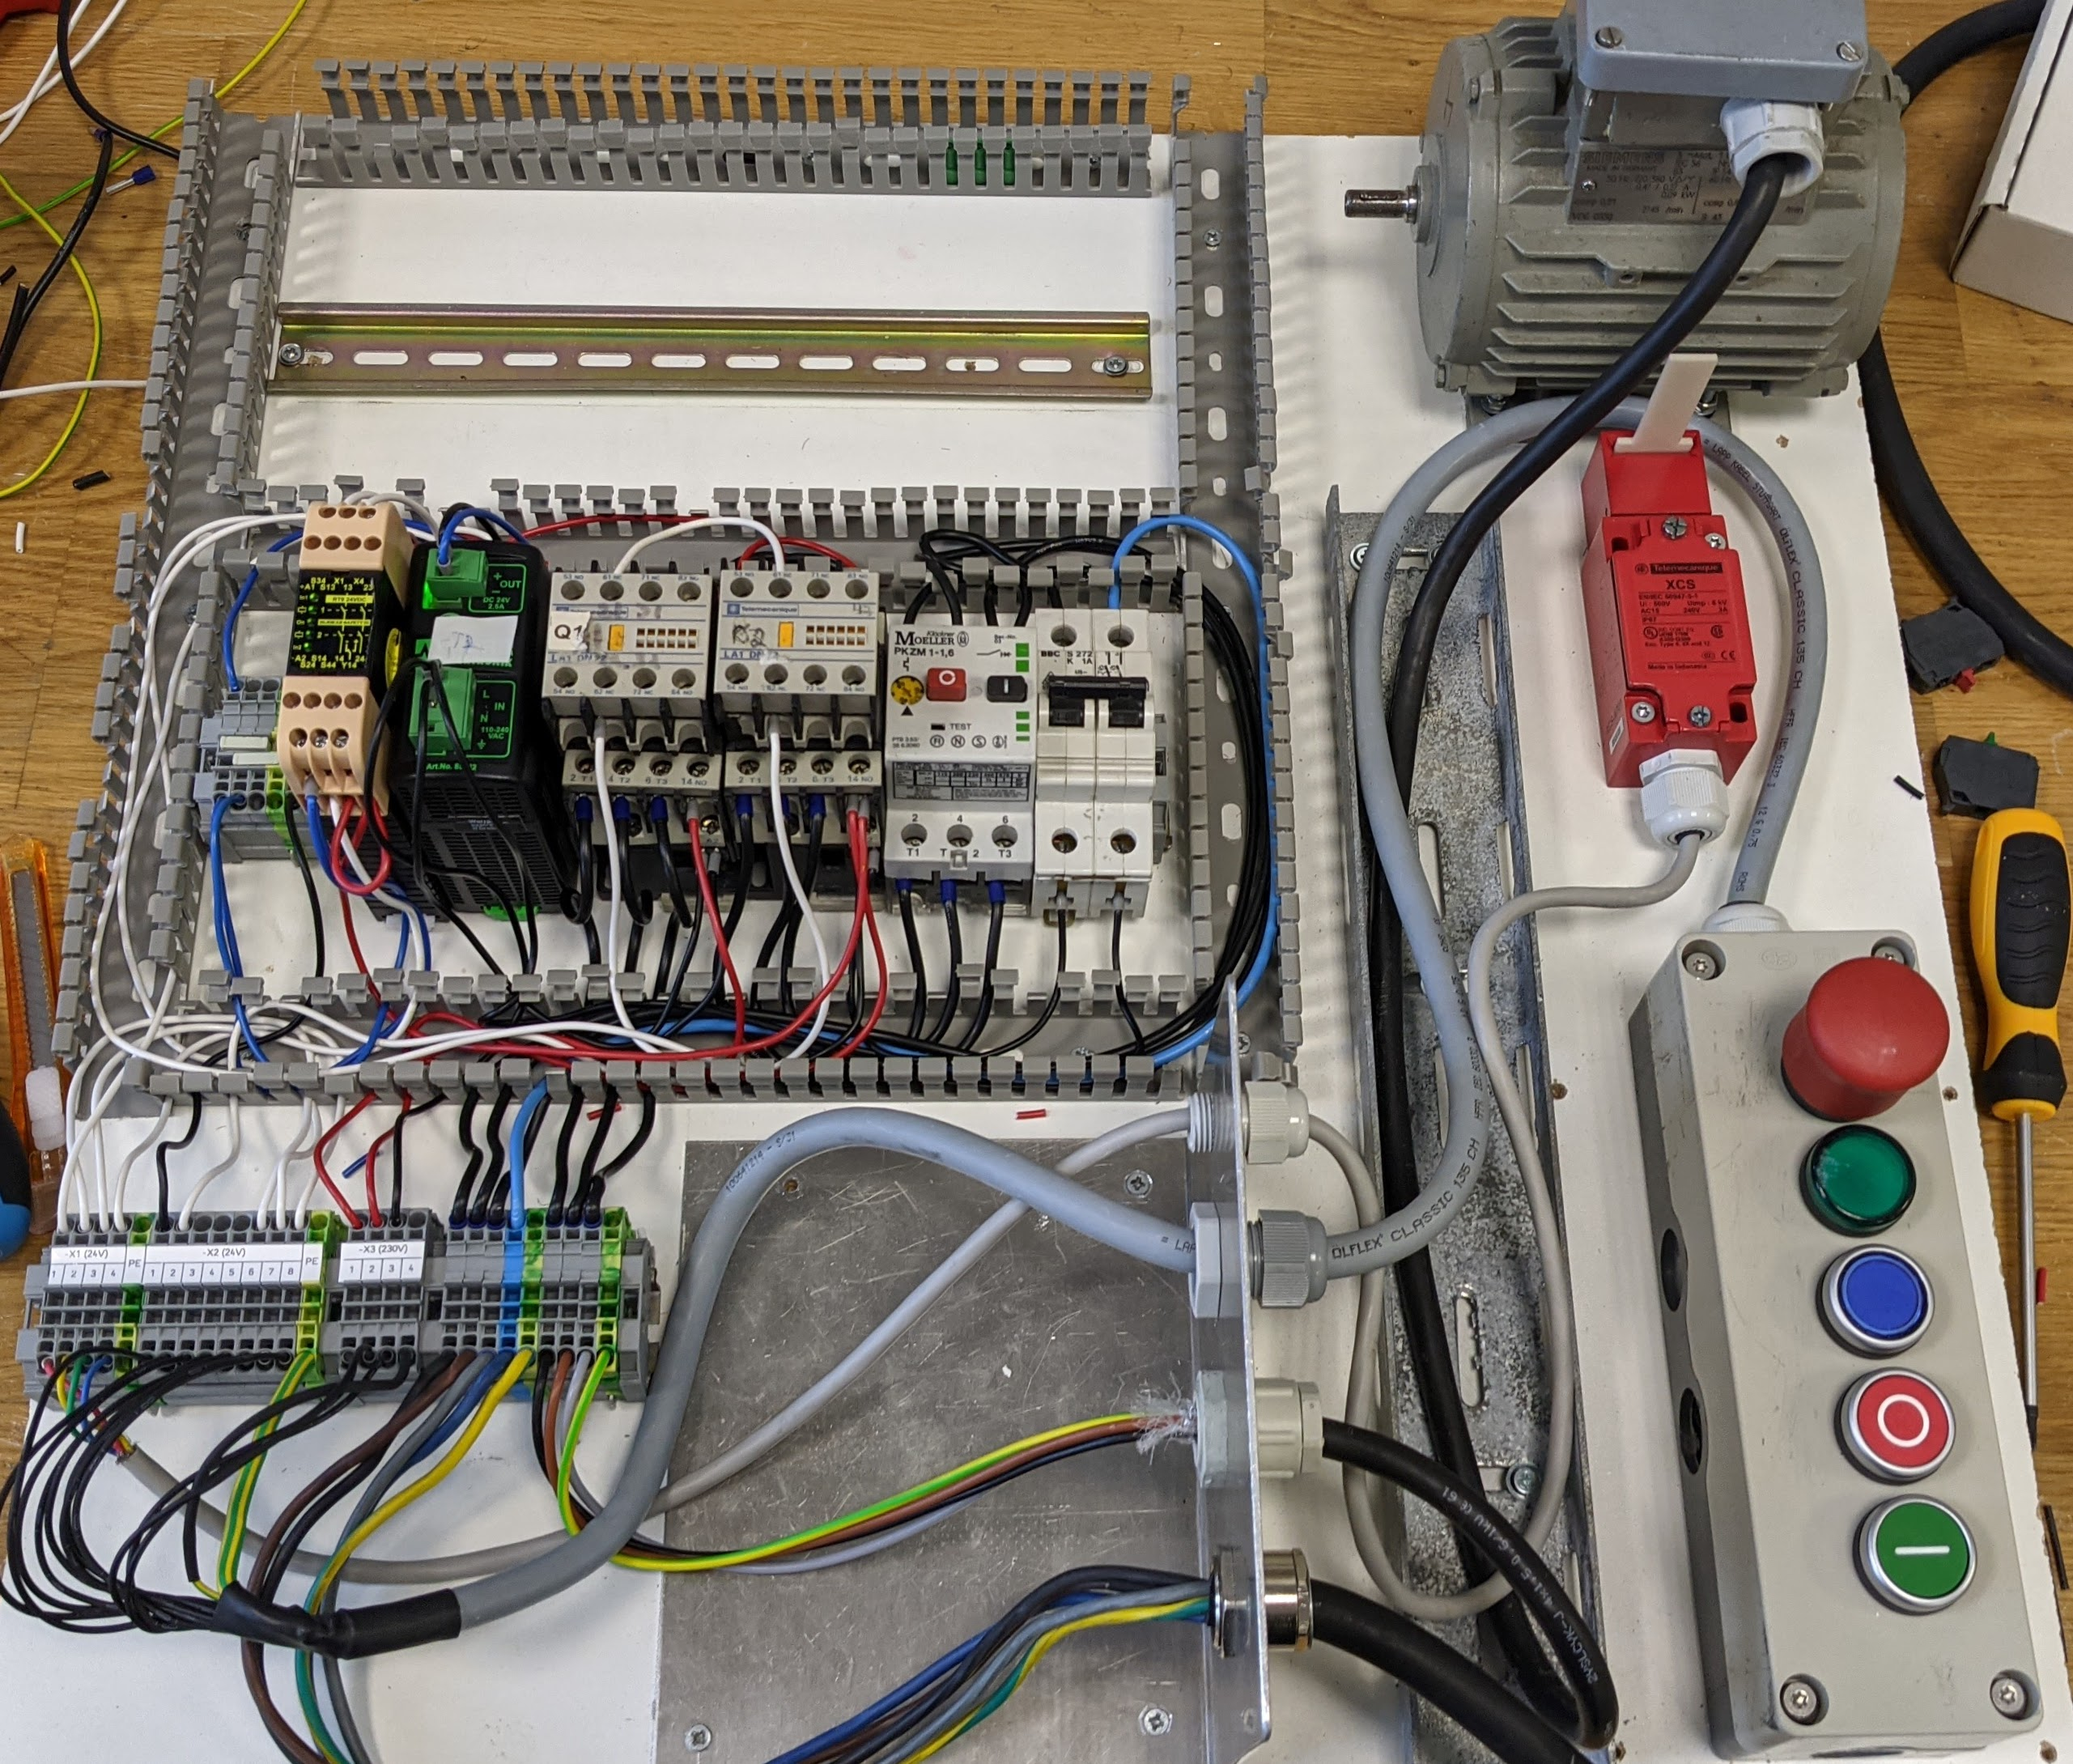
\includegraphics[width=13cm]{i04821x01.jpg}$$\\
















\underbar{file i04824}
\vfil \eject
%(END_QUESTION)





%(BEGIN_ANSWER)


%(END_ANSWER)





%(BEGIN_NOTES)


%INDEX% Arbeisdoppdrag, Styresystemer, Nivå 2, Stasjon03/04, Programmering av reguleringsstasjon

%(END_NOTES)


